\section{Benchmarks and results: Indexing}
\label{sec:benchmarks-indexing}

Indexing was measured at two levels: its CPU work alone with JMH on the host, and the whole path from
\code{index-queue} into MongoDB with the real services in Docker Compose. The scripts, the instructions to repeat every
measure and the raw results are in \code{benchmarks/indexing/}; the figures come from \code{benchmarks/plot.py}.

\subsection{Microbenchmarks with JMH}

The benchmarks live in the test code of \code{indexing-service}, package \code{...indexing.benchmark}, and run from the
benchmarks jar on the reference machine (Section~\ref{sec:consolidation}): 2 forks with a 4~GB heap, 5 warm-up and 10
measured iterations of 1~s each (20 samples), average time per operation with its 99.9~\% error. The books are three synthetic bodies of the dataset (short, median
and long), read from the page cache, so the benchmarks measure CPU, not disk.

\begin{table}[H]
\centering\small
\begin{tabularx}{\linewidth}{@{}Xrl@{}}
\toprule
\textbf{Benchmark} & \textbf{Time ($\mu$s)} & \textbf{Derived} \\
\midrule
Tokenize a short body (6.8~KB) & 114 $\pm$ 8 & 60 MB/s \\
Tokenize the median body (49.6~KB) & 844 $\pm$ 66 & 59 MB/s \\
Tokenize a long body (281.5~KB) & 5,137 $\pm$ 310 & 55 MB/s \\
Parse a header & 21.2 $\pm$ 0.7 & \\
Add a book to the pending posting lists, in memory & 1,320 $\pm$ 34 & \\
The same, pending map of the MongoDB index (nothing sent) & 1,343 $\pm$ 40 & \\
Prepare a batch of 100 books, per book, 1 thread & 4,297 $\pm$ 170 & 233 books/s \\
\quad 2 threads & 3,130 $\pm$ 126 & $\times$1.37 \\
\quad 4 threads & 2,119 $\pm$ 87 & $\times$2.03 \\
\quad 8 threads & 2,052 $\pm$ 39 & $\times$2.09 \\
\bottomrule
\end{tabularx}
\caption{JMH of the CPU part of indexing. A batch is read, parsed and tokenized on the parser threads; adding to the
posting lists stays in one thread.}
\label{tab:jmh-indexing}
\end{table}

The threads stop helping at 4: reading, parsing and tokenizing run in parallel, but adding to the posting lists is
serial and takes about 1.3~ms of the 2.1~ms per book. Even with 1 thread, the CPU work of a book (4.3~ms) is a small part
of the 66 to 500~ms that a book takes end to end, as the next section shows.

\subsection{Integration experiments}

\textbf{Method.} \code{run-experiments.sh} drives the real services of Docker Compose with the limits of \code{.env}:
Indexing with 2 CPUs and 1~GB, MongoDB with 2 CPUs, 1~GB and a WiredTiger cache of 0.25~GB. Each run starts clean: the
database is deleted and both Hazelcast members are restarted. With Indexing stopped, Ingestion puts the books of the
run in \code{index-queue}. Then Indexing starts at time 0, so its start-up counts, and the driver counts the
\code{INDEXED} books every second. \code{scripts/monitor.sh} samples the CPU and memory of every container every 2~s.
The Control is not started, because it would publish in the middle of a measure. The throughput is measured between 10
and 90~\% of the books, without the start-up and the last batch. Batches of 100 books; one factor changes at a time;
the books are the synthetic ones of the dataset, with real word frequencies. The whole run took 6.5~hours, and no book
ended \code{FAILED}.

\textbf{Threads.} 2,000 books, 1 replica, 3 repetitions each:

\begin{table}[H]
\centering\small
\begin{tabular}{@{}lrrrr@{}}
\toprule
\code{INDEXING\_THREADS} & \textbf{Books/s} & \textbf{Duration (s)} & \textbf{CPU Indexing} & \textbf{CPU MongoDB} \\
\midrule
1 & 14.87 $\pm$ 0.21 & 137.3 $\pm$ 2.5 & 14 \% & 101 \% \\
2 & 15.05 $\pm$ 0.15 & 135.7 $\pm$ 1.1 & 14 \% & 102 \% \\
4 & 15.14 $\pm$ 0.17 & 135.1 $\pm$ 1.2 & 14 \% & 104 \% \\
8 & 15.19 $\pm$ 0.24 & 134.7 $\pm$ 1.7 & 18 \% & 101 \% \\
\bottomrule
\end{tabular}
\caption{Indexing against its parser threads. CPU is the mean in \% of one core during the run. Peak memory: Indexing
476 to 477~MiB, MongoDB 538 to 582~MiB. Mean $\pm$ standard deviation of 3 runs.}
\label{tab:index-threads}
\end{table}

\begin{figure}[H]
\centering
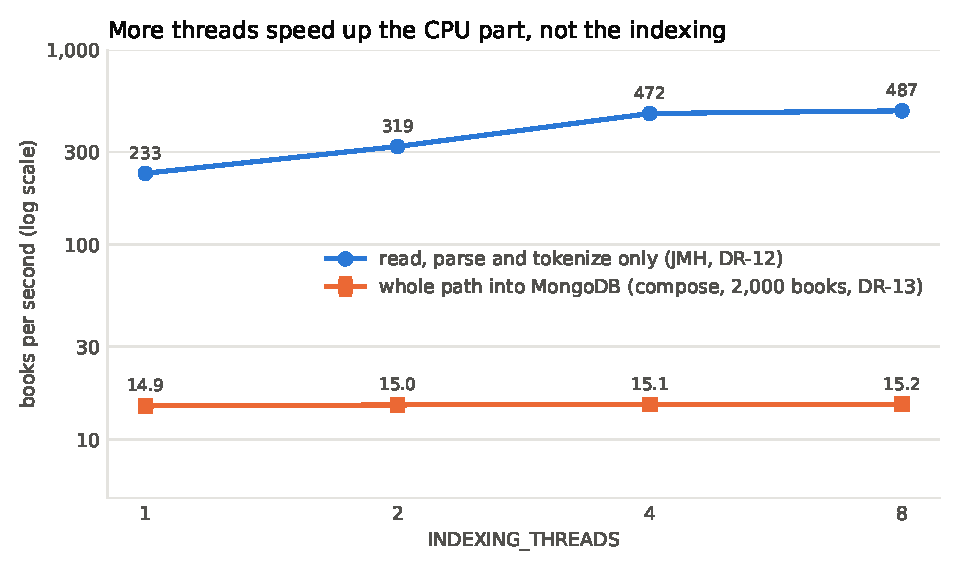
\includegraphics[width=0.49\linewidth]{figures/index_threads.pdf}\hfill
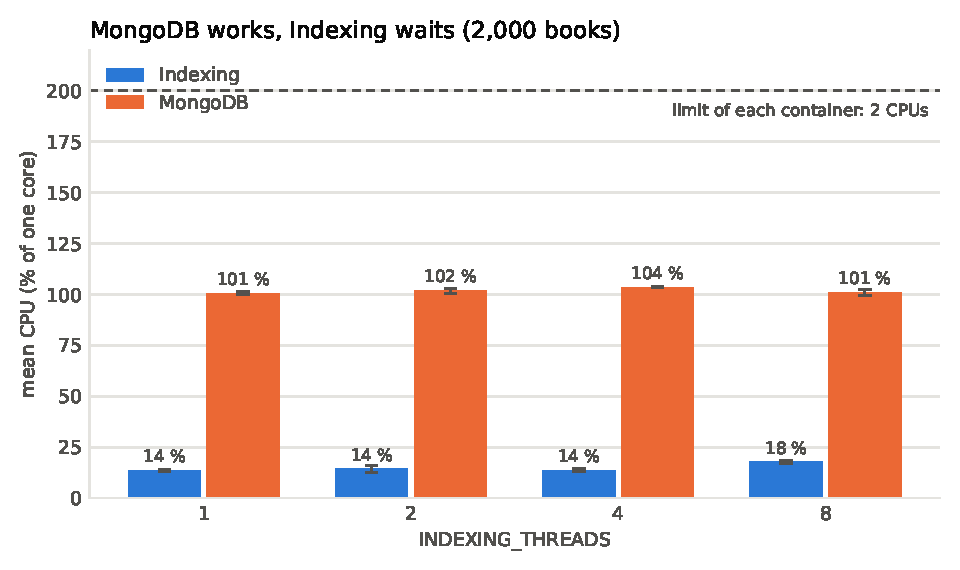
\includegraphics[width=0.49\linewidth]{figures/index_threads_cpu.pdf}
\caption{Left: books per second against the parser threads, for the CPU part alone (JMH) and for the whole path into
MongoDB. Right: mean CPU of Indexing and MongoDB in those runs.}
\label{fig:index-threads}
\end{figure}

\textbf{Scale.} 4 threads, 1 replica; 30,000 books ran once because one run takes more than 4~hours:

\begin{table}[H]
\centering\small
\begin{tabular}{@{}rrrrrrr@{}}
\toprule
\textbf{Books} & \textbf{Runs} & \textbf{Books/s} & \textbf{Duration} & \textbf{Terms} & \textbf{Index on disk} &
  \textbf{Longest list} \\
\midrule
200 & 3 & 24.90 $\pm$ 0.02 & 11 s & 58,244 & 5.8 MB & 200 ids \\
10,000 & 3 & 5.54 $\pm$ 0.01 & 30 min & 394,502 & 465 MB & 9,965 ids, 99 KB \\
30,000 & 1 & 2.00 & 4 h 10 min & 651,565 & 1.11 GB & 29,898 ids, 318 KB \\
\bottomrule
\end{tabular}
\caption{Indexing against the number of books. Peak memory: Indexing 404 to 518~MiB, MongoDB 461 to 802~MiB of its
1~GB, Hazelcast 326 to 390~MiB.}
\label{tab:index-scale}
\end{table}

\begin{figure}[H]
\centering
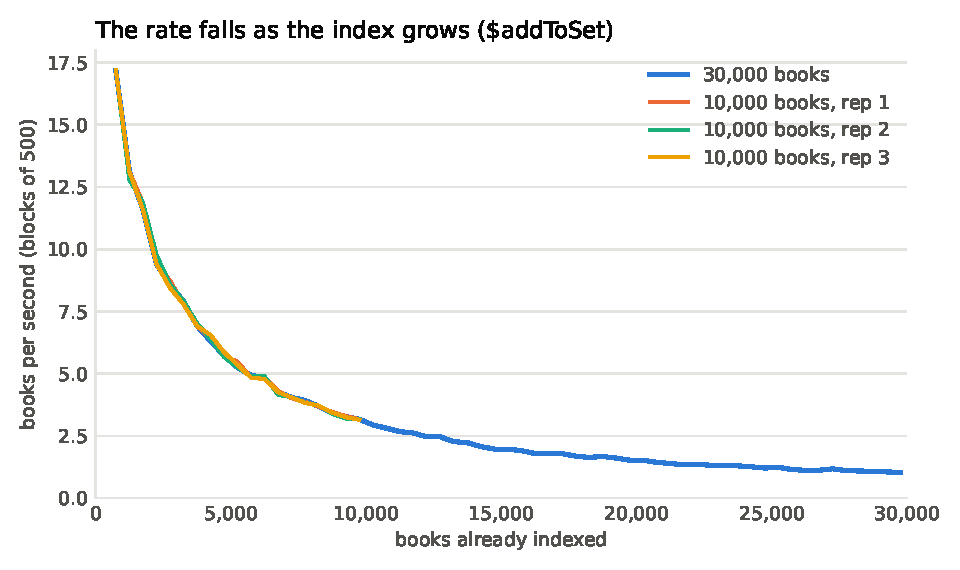
\includegraphics[width=0.75\linewidth]{figures/index_rate.pdf}
\caption{Books per second against the books already in the index, in blocks of 500 books (5 batches). The three runs
of 10,000 books and the run of 30,000 lie on one curve.}
\label{fig:index-rate}
\end{figure}

\textbf{Probe of the posting lists.} To isolate the cost of one update, the driver adds 100 ids to a single posting
list of a given length, 20 times, with \code{\$addToSet} and with \code{\$push}:

\begin{figure}[H]
\centering
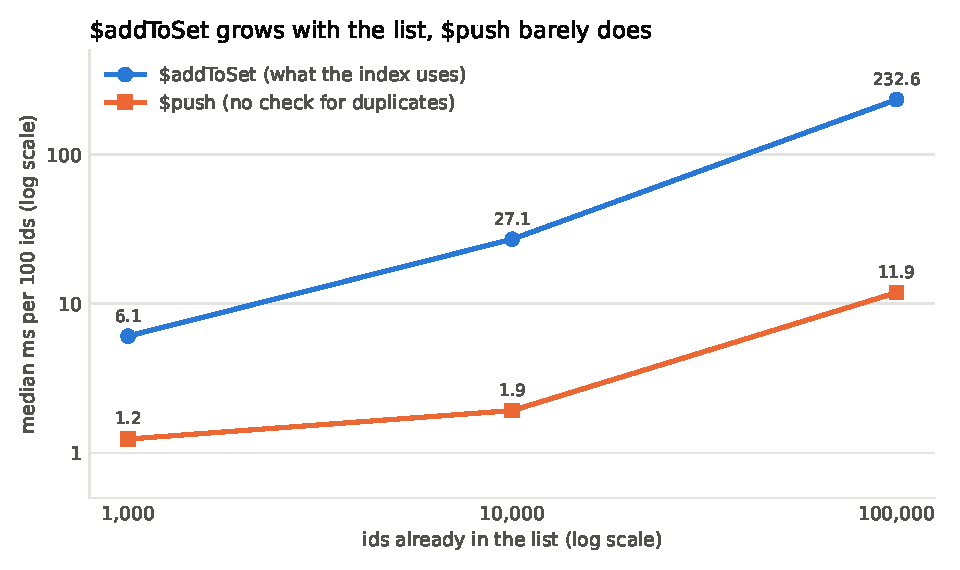
\includegraphics[width=0.49\linewidth]{figures/index_probe.pdf}\hfill
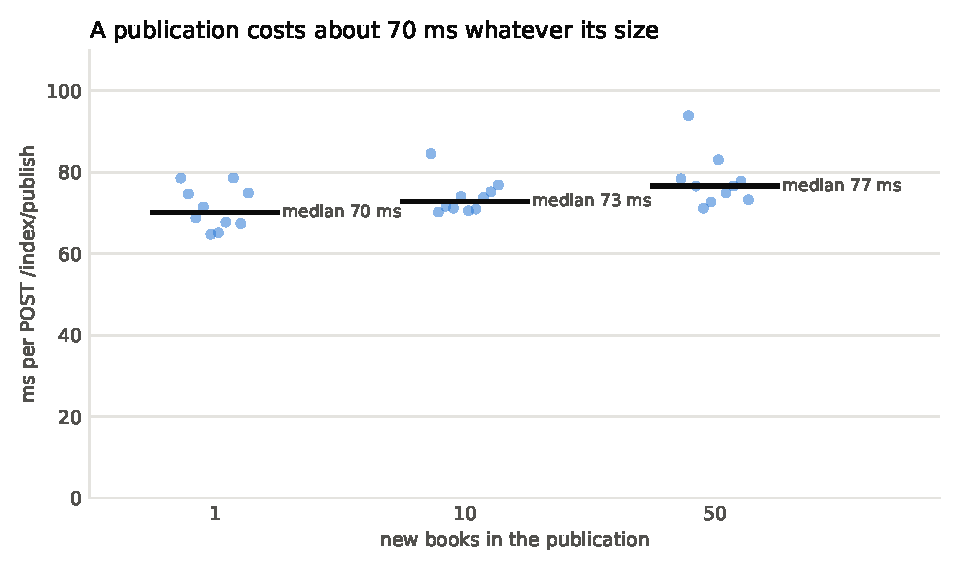
\includegraphics[width=0.49\linewidth]{figures/index_publish.pdf}
\caption{Left: median time to add 100 ids to one posting list. Right: each \code{POST /index/publish} of 1, 10 and 50
new books on an index of 10,000 books, 10 times each, and the median.}
\label{fig:index-probe-publish}
\end{figure}

\textbf{Publication.} \code{POST /index/publish} on an index of 10,000 books takes a median of 70, 73 and 77~ms for 1, 10
and 50 new books (Figure~\ref{fig:index-probe-publish}). The first publication, with all 10,000 books, took 459~ms.

\subsection{Analysis}

\begin{itemize}
  \item \textbf{Indexing is limited by MongoDB, not by its own CPU.} From 1 to 8 threads the rate improves by 2~\%,
        within the noise, while the CPU part alone doubles. Indexing uses less than a fifth of one core. MongoDB uses
        about one core of its two for the whole run, because a single writer sends one bulk write at a time: the work
        of MongoDB is one serial stream.
  \item \textbf{The rate falls as the index grows, and \code{\$addToSet} explains it.} At 10,000 books a batch of 100
        takes about 33~s, at 30,000 about 90~s. The probe shows why: \code{\$addToSet} compares each new id with the
        whole list, so its cost grows linearly with the list, 14 times that of \code{\$push} at 10,000 ids and 20 times
        at 100,000. The frequent terms hold almost one id per book, so every batch pays for the size of the index.
        The two scales agree where they overlap: books 9,000 to 12,000 of the 30,000 run went at 2.9 books/s, and the
        last tenth of the 10,000 runs at 3.2.
  \item \textbf{Publishing is cheap and its cost is fixed.} From 1 to 50 new books the median grows by 7~ms: the round
        trips of its steps dominate, not the books. The Control can therefore publish often, every 30~s or every 100
        books, without loading MongoDB.
  \item \textbf{Saturation point.} On this host and these limits, indexing does not saturate a resource of its own: it
        is bound by the time MongoDB takes per update, which grows with the index. Adding threads or replicas to
        Indexing changes nothing; changing the write (Section~\ref{sec:decisions-storage}) or giving MongoDB more cache
        and CPU would.
\end{itemize}

\textbf{Limits of these measures.}
\begin{itemize}
  \item Everything runs on one machine: the driver, \code{docker stats} and the services share its CPUs.
  \item The WiredTiger cache (0.25~GB) is smaller than the index from 10,000 books on. The probe isolates
        \code{\$addToSet} on one document, but in the full runs part of the slowdown may also come from the cache.
  \item MongoDB is not restarted between runs, only its database is deleted, so its peak memory grows along the run
        whatever the level.
  \item With 200 books only 1 or 2 samples of the monitor fall inside the run, so its CPU figures are not meaningful.
  \item 100,000 books were not measured: even at the rate of the last books of the 30,000 run, about one book per
        second and still falling, the 70,000 more books would take over 19~hours.
  \item Indexing replicas were not measured for throughput: by design only one writes. Their failover was measured
        (Section~\ref{sec:indexing}).
\end{itemize}
